%%%%%%%%%%%%%%%%%%%%%%%%%%%%%%%%%%%%%%%%%
% Journal Article
% LaTeX Template
% Version 1.4 (15/5/16)
%
% This template has been downloaded from:
% http://www.LaTeXTemplates.com
%
% Original author:
% Frits Wenneker (http://www.howtotex.com) with extensive modifications by
% Vel (vel@LaTeXTemplates.com)
%
% License:
% CC BY-NC-SA 3.0 (http://creativecommons.org/licenses/by-nc-sa/3.0/)
%
%%%%%%%%%%%%%%%%%%%%%%%%%%%%%%%%%%%%%%%%%

%----------------------------------------------------------------------------------------
%	PACKAGES AND OTHER DOCUMENT CONFIGURATIONS
%----------------------------------------------------------------------------------------

\documentclass[10pt]{article} % Single column

%\documentclass[twoside,twocolumn]{article} % Two column

\usepackage{blindtext} % Package to generate dummy text throughout this template 

\usepackage[sc]{mathpazo} % Use the Palatino font
\usepackage[T1]{fontenc} % Use 8-bit encoding that has 256 glyphs
\linespread{1.05} % Line spacing - Palatino needs more space between lines
\usepackage{microtype} % Slightly tweak font spacing for aesthetics

\usepackage[spanish,english]{babel} % Language hyphenation and typographical rules

\usepackage{algorithm}
	
\usepackage[hmarginratio=1:1,top=32mm,columnsep=20pt]{geometry} % Document margins
\usepackage[hang, small,labelfont=bf,up,textfont=it,up]{caption} % Custom captions under/above floats in tables or figures
\usepackage{booktabs} % Horizontal rules in tables

\usepackage{lettrine} % The lettrine is the first enlarged letter at the beginning of the text

\usepackage{enumitem} % Customized lists
\setlist[itemize]{noitemsep} % Make itemize lists more compact

\usepackage{abstract} % Allows abstract customization
\renewcommand{\abstractnamefont}{\normalfont\bfseries} % Set the "Abstract" text to bold
\renewcommand{\abstracttextfont}{\normalfont\small\itshape} % Set the abstract itself to small italic text

\usepackage{titlesec} % Allows customization of titles
\renewcommand\thesection{\Roman{section}} % Roman numerals for the sections
\renewcommand\thesubsection{\roman{subsection}} % roman numerals for subsections
\titleformat{\section}[block]{\large\scshape\centering}{\thesection.}{1em}{} % Change the look of the section titles
\titleformat{\subsection}[block]{\large}{\thesubsection.}{1em}{} % Change the look of the section titles

\usepackage{fancyhdr} % Headers and footers
\pagestyle{fancy} % All pages have headers and footers
\fancyhead{} % Blank out the default header
\fancyfoot{} % Blank out the default footer
\fancyhead[C]{Aprendizaje de M\'aquinas \textbf{Descubrimiento de Conocimiento M\'edico}} % Custom header text
\fancyfoot[RO,LE]{\thepage} % Custom footer text

\usepackage{titling} % Customizing the title section

\usepackage{hyperref} % For hyperlinks in the PDF

\usepackage{graphicx} % For images

\usepackage{pifont} % bullets

\usepackage{amsmath}

\usepackage{algpseudocode}

\usepackage{multirow}

% Keywords command
\providecommand{\keywords}[1]
{
	\small	
	\vspace{0.5em}
	\noindent \textbf{\textit{Palabras clave --- }} #1
}


%----------------------------------------------------------------------------------------
%	TITLE SECTION
%----------------------------------------------------------------------------------------

\setlength{\droptitle}{-4\baselineskip} % Move the title up

\pretitle{\begin{center}\Huge\bfseries} % Article title formatting
	\posttitle{\end{center}} % Article title closing formatting
\title{\normalsize{Aprendizaje de M\'aquinas}\\
	\Huge\bfseries Descubrimiento de Conocimiento M\'edico \\
} % Article title
\author{% 
	Diamis Alfonso \\ Mari\'e del Valle \\ Roxana Pe\~na \\ Dennis Fiallo \\ Ernesto Alfonso \\ Rolando Sanch\'ez
	Ro \vspace{1em} \\
	\small Cuarto a\~no. Ciencias de la Computaci\'on. \\ % institution
	\small Facultad de Matem\'atica y Computaci\'on, Universidad de La Habana, Cuba \\ % institution
}
\date{} % Leave empty to omit a date


% Abstract configurations
\renewenvironment{abstract}
{\small
	\begin{center}
		\bfseries \abstractname\vspace{-.5em}\vspace{0pt}
	\end{center}
	\list{}{
		\setlength{\leftmargin}{1.5cm}%
		\setlength{\rightmargin}{\leftmargin}%
	}%
	\item\relax}
{\endlist}

\usepackage{amsthm}
\usepackage{amssymb}
\usepackage{todonotes} % \TODO
\usepackage{listings} % Code listings
\usepackage{xcolor}

\definecolor{backcolour}{rgb}{0.95,0.95,0.92}

\newcommand{\csl}[1]{\colorbox{backcolour}{\texttt{#1}}}

\newcommand{\imgcaption}[2]{\tiny \textbf{Figura #1.} #2.}

\newcommand{\mgc}[2][]{\colorbox{backcolour}{\texttt{\_\_#2\_\_#1}}}

\newcommand{\mgccapt}[1]{\texttt{\_\_#1\_\_}}

\newtheorem{thm}{Teorema}
\newtheorem{mydef}{Definici\'on}%[section]
\newtheorem{lem}{Lema}
\newtheorem{fig}{\scriptsize{Figura}}
\newtheorem{col}{Corolario}

\renewcommand{\qedsymbol}{\rule{0.7em}{0.7em}}

% Hyperlinks configurations
\hypersetup{
	colorlinks=true,
	linkcolor=black,
	filecolor=magenta,      
	urlcolor=cyan,
	pdftitle={Overleaf Example},
	pdfpagemode=FullScreen,
}

%----------------------------------------------------------------------------------------

\begin{document}
	% Print the title
	\maketitle
	
	%----------------------------------------------------------------------------------------
	%	ARTICLE CONTENTS
	%----------------------------------------------------------------------------------------
	\selectlanguage{spanish}
	\begin{abstract}		
		En este estudio, abordamos el desafío de la extracción de conocimiento a partir de textos médicos mediante la identificación de entidades, su clasificación y la detección de relaciones entre ellas. Para llevar a cabo estas tareas de Extracción de Entidades Nombradas (NER) y Extracción de Relaciones (RE), experimentamos con diversos modelos de procesamiento del lenguaje natural como BiLSTM, BERT, T5 y GPT3. A través de nuestras pruebas comparativas, encontramos que T5 demostró ser el modelo más robusto para estas tareas, superando a los demás en términos de precisión y eficiencia. Además, para maximizar la utilidad de los conocimientos extraídos, desarrollamos una ontología en una base de datos en formato de grafo utilizando Neo4J. Este recurso proporciona una plataforma para la exploración y el uso futuro de los resultados inferidos, potenciando la accesibilidad y aplicabilidad de los valiosos conocimientos extraídos de los textos médicos.	
	\end{abstract}

	\selectlanguage{english}
	\begin{abstract}		
	In this study, we tackle the challenge of knowledge extraction from medical texts by identifying entities, their classification, and detecting relationships between them. To perform these Named Entity Recognition (NER) and Relation Extraction (RE) tasks, we experimented with various natural language processing models such as BiLSTM, BERT, T5, and GPT3. Through our comparative tests, we found that T5 proved to be the most robust model for these tasks, surpassing others in terms of accuracy and efficiency. Furthermore, to maximize the utility of the extracted knowledge, we developed an ontology in a graph-formatted database using Neo4J. This resource provides a platform for the exploration and future use of the inferred results, enhancing the accessibility and applicability of the valuable knowledge extracted from medical texts.
	\end{abstract}

	\section{Repositorio del proyecto}
	
	\begin{center}
		\href{https://github.com/computer-science-crows/algorithms-design-and-analysis}{https://github.com/computer-science-crows/algorithms-design-and-analysis}
	\end{center}

	\section{Introducci\'on}
	
	La era digital actual ha llevado a un crecimiento explosivo en la generación y disponibilidad de datos, especialmente en el campo de la medicina. Sin embargo, la mayoría de estos datos son textos no estructurados que requieren métodos de procesamiento sofisticados para extraer conocimientos valiosos. Es en este contexto que surge el desafío que abordamos en este trabajo: la extracción de conocimiento a partir de textos médicos.
	% mediante la identificación de entidades y la detección de relaciones entre ellas.
	
	En la literatura científica, se han propuesto diversos enfoques para abordar este problema, que abarcan desde métodos basados en reglas hasta enfoques de aprendizaje supervisado y no supervisado. Sin embargo, el surgimiento de técnicas de procesamiento de lenguaje natural (NLP) basadas en aprendizaje profundo ha abierto nuevas puertas para la extracción de conocimientos de textos médicos. \todo{Mencionar primero que el enfoque fue NER y RE} Específicamente, los modelos como BiLSTM, BERT, T5, y GPT3 han demostrado ser particularmente efectivos para los problemas de Extracción de Entidades Nombradas (NER) y Extracción de Relaciones (RE). 
	
	En este trabajo, experimentamos con estos modelos y evaluamos su rendimiento en la tarea de extracción de conocimiento de textos médicos. Nuestra investigación se enfocó en identificar qué modelo es el más robusto y efectivo para estas tareas. Además, para facilitar el uso futuro de los conocimientos extraídos, desarrollamos una ontología en una base de datos en formato de grafo usando Neo4J. Esta ontología no solo almacena las entidades y relaciones identificadas, sino que también permite consultas complejas y análisis de red, abriendo nuevas posibilidades para el uso de los datos.
	
	Este trabajo aporta una contribución valiosa al campo de la extracción de conocimiento de textos médicos, no solo al evaluar el rendimiento de varios modelos de NLP de vanguardia, sino también al proponer una forma novedosa de almacenar y utilizar los conocimientos extraídos. Creemos que nuestros hallazgos serán de interés para los investigadores y profesionales que trabajan en la intersección de la medicina, la informática y la inteligencia artificial.
	
	\section{Estado del Arte}
	\todo{(AGREGAR REFERENCIA!!)}
	\todo{Buscar estado del arte en el descubrimiento de conocimiento}
	El Estado del Arte en la extracción de entidades y relaciones de textos médicos ha avanzado rápidamente en los últimos años gracias a los avances en el Procesamiento de Lenguaje Natural (NLP) y en particular, al aprendizaje profundo.
	
	La Extracción de Entidades Nombradas (NER) ha sido una tarea fundamental en NLP durante mucho tiempo. Los enfoques tradicionales solían incluir técnicas basadas en reglas y métodos de aprendizaje automático supervisado que utilizaban características manuales. Sin embargo, con el advenimiento del aprendizaje profundo, los modelos basados en redes neuronales recurrentes (RNN) como LSTM y GRU han mostrado un rendimiento impresionante en tareas de NER. En particular, el modelo BiLSTM, que procesa la secuencia de entrada en ambas direcciones, ha sido ampliamente utilizado para tareas de NER debido a su capacidad para capturar el contexto de ambas direcciones.
	
	Para la tarea de Extracción de Relaciones (RE), los modelos basados en Transformadores, como BERT de Google, han demostrado ser particularmente eficaces. BERT presenta una nueva arquitectura que se basa en la atención de múltiples cabezas y ha demostrado tener un rendimiento superior en varias tareas de NLP, incluyendo RE. Otra variante, BioBERT, un modelo preentrenado en textos biomédicos, ha obtenido resultados aún mejores en las tareas de RE en el dominio médico.
	
	En cuanto a los conjuntos de datos para la evaluación de estas tareas, se han utilizado varios corpus en la literatura. Un ejemplo notorio es el corpus eHealth-KD, que proporciona un conjunto de datos anotados en el dominio de la salud. Este conjunto de datos incluye entidades y relaciones etiquetadas, y ha sido utilizado en varias competencias científicas para evaluar el rendimiento de diferentes enfoques para las tareas de NER y RE.
	
	Además de eHealth-KD, existen otras bases de datos relevantes como SemEval, BioNLP, i2b2, y MIMIC-III, que son ampliamente utilizadas en el campo del procesamiento de texto biomédico y médico. Estos conjuntos de datos, que varían en tamaño, complejidad y enfoque, proporcionan una amplia gama de contextos para probar y evaluar métodos de NER y RE.
	
	En resumen, el estado del arte en la extracción de entidades y relaciones de textos médicos está dominado por los enfoques de aprendizaje profundo, con modelos como BiLSTM y BERT que ofrecen un rendimiento superior. Sin embargo, la elección del modelo adecuado puede depender del contexto específico y del conjunto de datos disponibles, y la investigación en este campo sigue siendo un área activa y en evolución.
	
	
	\section{Datos}
	\todo{Mencionar los tipos de entidades y de relaciones}
	El dataset utilizado en nuestro proyecto se basó en el corpus \todo{(AGREGAR REFERENCIA!!)}. Este dataset tiene las siguientes características:
	
	- Es multidominio y multilingüe, lo que significa que abarca una variedad de temas relacionados con la salud y contiene oraciones en diferentes idiomas.
	- Todas las oraciones del dataset están relacionadas con temas de salud, lo que proporciona una gran variedad en términos de formato y estructura.
	- Cada oración del dataset está etiquetada, lo que significa que se conoce el dominio al que pertenece y el idioma correspondiente.
	- En el conjunto de entrenamiento, se tienen un total de 1400 oraciones, de las cuales 1200 están en español y 200 en inglés.
	- En el conjunto de pruebas, se tienen un total de 100 oraciones, de las cuales 75 están en español y 25 en inglés.
	- Para evaluar la extracción de entidades, se utilizó un coeficiente de Gini de 0.39, lo que indica un rendimiento moderado en esta tarea.
	- Para evaluar la extracción de relaciones, se utilizó un coeficiente de Gini de 0.58, lo que indica un rendimiento más alto en esta tarea.
	
	Este dataset proporciona una base sólida para el entrenamiento y evaluación de modelos de extracción de conocimiento en el campo de la salud, con una variedad de oraciones etiquetadas en diferentes idiomas y dominios.
	
	En el proyecto contamos con cuatro tipos de entidades:
	\begin{itemize}
		\item Concept: identifica un término relevante, concepto, idea, en el dominio de conocimiento de la oración.
		\item Action: identifica un proceso o modificación de otras entidades. Puede ser indicado por un verbo o construcción verbal, como “afecta” (afecta), pero también por sustantivos, como “exposición”, donde denota el acto de estar expuesto al sol, y “daños” (daños), donde denota el acto de dañar la piel. También se puede utilizar para indicar relaciones funcionales no verbales, como “padre”, etc.
		\item Predicate: identifica una función o filtro de otro conjunto de elementos, que tiene una etiqueta semántica en el texto, como “mayores” (mayores), y se aplica a una entidad, como “personas” (personas) con algunos argumentos adicionales como “60 años” (60 años).
		\item Reference: identifica un elemento textual que hace referencia a una entidad –de la misma oración o de otra diferente–, lo que puede indicarse mediante claves textuales como “esta”, “aquel”, etc.
	\end{itemize}
	
	Y las relaciones:
	
	\begin{itemize}
		\item is-a: indica que una entidad es un subtipo, instancia o miembro de la clase identificada por la otra.
		\item same-as: indica que dos entidades son semánticamente iguales.
		\item has-property: indica que una entidad tiene una determinada propiedad o característica.
		part-of: indica que una entidad es parte constitutiva de otra.
		\item  causes: indica que una entidad provoca la existencia o ocurrencia de otra.
		\item entails: indica que la existencia de una entidad implica la existencia o ocurrencia de otra.
		\item in-time: para indicar que algo existe, ocurre o está confinado a un marco de tiempo, como en “exposición” in-time “verano”.
		\item in-place: para indicar que algo existe, ocurre o está confinado a un lugar o ubicación.
		\item in-context: para indicar un contexto general en el que sucede algo, como un modo, manera o estado, como “exposición” en contexto “prolongada”.
		\item subject: indica quién realiza la acción, como en “[el] asma afecta […]”.
		\item target: indica quién recibe el efecto de la acción, como en " [...] afecta [las] v\'ias respitatorias". Las acciones pueden tener varios sujetos y destinatarios, en cuyo caso la semántica interpretada es que la unión de los sujetos realiza la acción sobre cada uno de los destinatarios.
		\item domain: indica la entidad principal sobre la que se aplica el predicado.
		\item arg: indica una entidad adicional que especifica un valor para que el predicado tenga sentido. La semántica exacta de este argumento depende de la semántica de la etiqueta del predicado, como en “mayores [de] 60 años”, donde la etiqueta del predicado “mayores” indica que “60 años” es una cantidad que restringe la edad mínima para el predicado sea verdadero.
		
	\end{itemize}
	
	\section{Propuesta}
	\todo{Poner un parrafito aqui}
	\subsection{BiLSTM} 
	Una solución para ambas tareas se basa en Redes Neuronales Recurrentes (RNN) o, más precisamente, en Memoria a Largo Plazo Bidireccional (BiLSTM) como codificadores contextuales y capas densas como la arquitectura del decodificador de etiquetas del modelo. Esta arquitectura es elegida debido a la estructura secuencial de la entrada y es ampliamente utilizada en la literatura \todo{poner referencia} para abordar el problema del Reconocimiento de Entidades Nombradas (NER). El sistema utiliza información de etiquetas POS (Part-of-Speech tag), relaciones de dependencia, representaciones a nivel de caracteres, así como incrustaciones contextuales. La tarea de Extracción de Relaciones (RE) se aborda de manera pareada, codificando la información sobre la oración y el par de entidades dado utilizando estructuras sintácticas derivadas del árbol de análisis de dependencia. Además, se utilizó un tipo especial de relación para codificar la relación entre pares de entidades no relacionadas.
	
	\subsubsection{Implementaci\'on} 
	La solución propuesta resuelve ambas tareas de manera separada y secuencial. Por lo tanto, se entrenaron modelos independientes con diferentes arquitecturas y características para resolver los problemas de NER y RE. La principal distinción entre las dos arquitecturas surge del tipo de problema que resuelven. 
	
	El primer problema (NER) se plantea como un problema de predicción de etiquetas que toma el texto sin procesar de una oración como entrada y genera dos secuencias de etiquetas independientes: una en el sistema de etiquetas BILOUV para la predicción de entidades y otra con las etiquetas correspondientes a cada tipo de entidad. La clasificación del esquema de etiquetas BILOUV corresponde a \textit{Begin}, para el inicio de una entidad; \textit{Inner}, para el token en medio; \textit{Last}, para el token final; \textit{Unit}, para representar entidades de un solo token; \textit{Other} para representar tokens que no pertenecen a ninguna entidad, y la etiqueta \textit{oVerlapping}\todo{se escribe as\'i?} se utiliza para lidiar con tokens que pertenecen a múltiples entidades. Por otro lado, el segundo problema (RE) se aborda como una serie de consultas por pares entre las entidades presentes en la oración objetivo, orientada a identificar las relaciones relevantes entre las entidades previamente extraídas. 
	
	Teniendo en cuenta las características multilingües de la tarea, el proceso de extracción de características de las características sintácticas se maneja en dos fases. En la primera, la oración de entrada se clasifica por su idioma utilizando un modelo preentrenado de FastText para la identificación del idioma. Posteriormente, en la segunda fase, se utilizaron dos modelos diferentes de Spacy (\url{https://spacy.io/}) dependiendo del idioma de la oración (es core news sm para español y en core web sm para inglés). Estos modelos se utilizaron para extraer características como la etiqueta POS, el árbol de análisis de dependencia y la etiqueta de dependencia.
	
	\subsection{BERT}
	
	En la actualidad, BERT (Bidirectional Encoder Representations from Transformers) se considera uno de los modelos de lenguaje más avanzados en NLP debido a su capacidad para capturar el contexto bidireccional de las palabras en una oración o secuencia de texto. Esto permite comprender mejor las relaciones y significados de las palabras en un contexto específico, lo que resulta beneficioso para tareas como la NER en el campo médico.
	
	\subsubsection{Implementaci\'on}
	En el proyecto, se siguió el siguiente método para ajustar el modelo BERT y abordar la tarea de NER en el conjunto de datos médicos eHealthKD2021:
	
	\begin{enumerate}
		\item Preprocesamiento de datos: Los datos de eHealthKD2021 se prepararon para que fueran compatibles con el formato de entrada requerido por BERT. Se tokenizó el texto y se agregaron los marcadores especiales [CLS] (inicio) y [SEP] (final). Además, se aplicaron técnicas de tokenización para dividir las palabras en subunidades más pequeñas y mejorar la capacidad del modelo para identificar entidades.
		
		\item Ajuste del modelo BERT: Se utilizó una implementación preentrenada de BERT y se ajustaron los hiperparámetros para adaptar el modelo a la tarea de NER con los datos médicos. Se seleccionó la arquitectura BERT apropiada y se configuraron los hiperparámetros, como la tasa de aprendizaje y el tamaño del lote. El modelo se entrenó utilizando el conjunto de datos de entrenamiento durante 2 epochs (épocas) para ajustar los pesos y mejorar su rendimiento en la tarea de NER.
		
		\item Evaluación del modelo: Una vez ajustado el modelo, se evaluó su desempeño utilizando el conjunto de datos de prueba. Se utilizaron métricas estándar de evaluación de NER, como precisión, recobrado y F1, descritas en las f\'ormulas \todo{refenrenciar f\'ormulas}
	\end{enumerate}
	
	\subsection{T5}
	
	T5, que significa "Text-to-Text Transfer Transformer", es un modelo de procesamiento de lenguaje natural desarrollado por Google. La idea principal detrás de T5 es tratar todas las tareas de NLP como un problema de generación de texto. Esto significa que tanto la entrada como la salida del modelo son siempre texto.
	
	El modelo T5 se entrena en un objetivo de "\textit{denoising}", es decir, se le dan cadenas de texto con ruido (por ejemplo, palabras borradas o enmascaradas) y se le pide que genere el texto original. Este enfoque es similar a otros modelos basados en transformadores como BERT, pero a diferencia de BERT y otros, T5 se entrena para generar cualquier tipo de texto, no sólo completar los espacios en blanco.
	
	El T5 es un modelo de "\textit{transformador}", lo que significa que utiliza la arquitectura del transformador introducida en el paper \todo{referenciar paper "Attention is All You Need" de Vaswani et al. (2017).} Esta arquitectura se basa en mecanismos de "\textit{atención}" que permiten al modelo ponderar diferentes partes del texto de entrada cuando genera la salida, lo que le permite capturar relaciones a largo plazo en el texto.
	
	Una de las ventajas clave del modelo T5 es su versatilidad. Debido a su enfoque de "texto a texto", puede ser utilizado para una amplia gama de tareas de NLP, incluyendo traducción de lenguaje, generación de resúmenes, respuesta a preguntas, y muchas otras, simplemente cambiando la forma en que se formatea la entrada.
	
	El T5 ha demostrado ser un modelo muy poderoso y ha obtenido resultados de vanguardia en una variedad de tareas de benchmarking de NLP. Sin embargo, al igual que otros modelos de gran tamaño, requiere una gran cantidad de recursos computacionales para entrenar y utilizar. A pesar de este desafío, el T5 representa un avance significativo en el campo de NLP y continúa influenciando el desarrollo de nuevos modelos y técnicas.
	
	\subsubsection{Implementaci\'on}
	\todo{Poner p\'arrafo de lo que se hace en la secci\'on}
	\textbf{NER}
	\vspace{0.5em}
	
	El archivo \textit{models/T5/NER\_T5\_spacy.ipynb} contiene el pipeline de la propuesta de soluci\'on al problema de reconocimiento de entidades y su clasificaci\'on. Para llegar a la soluci\'on se divide el problema en dos partes:
	\begin{enumerate}
		\item Dada una oraci\'on (en ingl\'es o espa\~nol) detectar las entidades.
		\item Dada una entidad, decir el tipo de esta.
	\end{enumerate}
		
	Para el primer paso nos apoyamos en la libreria \textit{Spacy} de Python y descargamos los m\'odulos de ambos idiomas. Esta librer\'ia devuelve una lista de todos los t\'erminos de la oraci\'on con sus respectivas clasificaciones.
	Estas clasificaciones no son las mismas que las de nuestro modelo, as\'i que se modifican las  entidades de \textit{Spacy} que son necesarias en la su resoluci\'on. Luego, para el segundo paso se utiliza el modelo \textit{Simple T5} y se entrena (con 5 epoch) para que sea capaz de clasificar las entidades.
	
	En el pipeline se calcula la efectividad de nuestro modelo de forma separada y junta, es decir, calculando la precisi\'on, el recobrado y la puntuación F1 se pueden observar las estad\'isticas de cu\'an exacto es \textit{Spacy} para el paso 1 y cu\'anto lo es T5 para el paso 2. Luego, se unen ambos m\'etodos para resolver la el problema NER como un todo.
	
	\textbf{RE}
	\vspace{0.5em}
	
	El archivo \textit{models/T5/SimpleT5\_RE\_CLF\_eHealthKD.ipynb} se encuentra la propuesta del modelo Transformer T5 para la tarea de extracción de relaciones.
	 	
	En un inicio, el modelo realizaba un entrenamiento supervisado en el que se le pasaba las entidades y el tipo de relación que existía entre ellas. Pero este enfoque en entrenamiento no dió los resultados esperados, pues en dependencia del contexto de la oración podría cambiar el tipo de relación entre las entidades.
	
	Para solucionar este problema se decidió cambiar el tipo de entrada del modelo, de forma tal que, por cada oración, se genera un conjunto de oraciones de entrenamiento para cada par de entidades posibles, con dichas  entidades marcadas (en forma de etiquetas como HTML). La salida del modelo es el tipo de relación. De esta manera, el modelo es entrenado para predecir el tipo de relación entre dos entidades dadas, basándose en el contexto de la oración, con lo cual un mejor desempeño en la soluci\;on del problema, duplicando la puntuación F1 del modelo.
	
	Se usa la técnica de Transfer Learning para entrenar, usando el modelo pre-entrenado "\textit{t5-base}", el segundo de 5 en la escala de tamaño de los modelos T5. Además se realizan 4 epochs de entrenamiento, en los cuales se mostraba una mejora de los resultados, pero no se siguió probando en adelante debido a falta de poder de computo y lo costoso que es el entrenamiento en cuanto a tiempo.
	
	%Se puede encontrar el pipeline de la propuesta de solución en el archivo \textit{pipeline\_lstm\_NER\_T5\_RE.ipynb}.
	\subsection{GPT3}
	
	La \'ultima soluci\'on implementada se realiz\'o utilizando GPT3, el modelo generativo preentrenado de OpenAI, en combinación con LangChain, una herramienta que facilita el procesamiento del lenguaje natural. GPT3 es una evolución del modelo Transformer, que se basa en la idea de predecir palabras en una secuencia de texto. Aunque GPT3 se ha usado principalmente para generación de texto, también puede ser muy efectivo en tareas de clasificación y etiquetado, como la extracción de entidades nombradas (NER) y la extracción de relaciones (RE). LangChain, por otro lado, es una herramienta que facilita la interacción con estos modelos de lenguaje, proporcionando una interfaz intuitiva para analizar y manipular texto. Su integración con GPT3 permite aprovechar la capacidad del modelo para reconocer y entender patrones en los datos de texto.
	
	\todo{Mejorar esto}
	Para la tarea de NER, se utiliza GPT3 para etiquetar las entidades en el texto. Este modelo es capaz de entender el contexto de cada palabra en una secuencia, lo que le permite identificar correctamente las entidades, incluso cuando la misma palabra puede tener diferentes significados en diferentes contextos.
	
	Para la tarea de RE, aplicamos GPT3 de manera similar, pero en este caso, buscamos relaciones entre las entidades identificadas. GPT3 puede identificar estas relaciones gracias a su capacidad para entender la semántica del texto.
	
	\subsection{Ontolog\'ias}
	
	En nuestro proyecto, una vez obtenido todo el conociemto de los documentos se guardan los datos en una base de datos orientada a grafos (BDOG). Dicha base de datos, representa las entidades como nodos de un grafo y sus relaciones con las aristas del mismo, de manera que se pueda usar teoría de grafos para recorrer la base de datos, ya que esta puede describir atributos de los nodos y las aristas.
	
	Para su implementaci\'on se utiliza \textit{Neo4j},  una base de datos altamente escalable y no estructurada (NoSQL), lo cual permite acceder a los datos de diversas formas y usando distintos lenguajes de consulta. El lenguaje usado para consultar y manipular los grafos es \textit{Cypher}. Este lenguaje es como SQL para grafos, y se inspiró en SQL, por lo que le permite concentrarse en los datos que desea obtener del grafo (no en cómo obtenerlos). Adem\'as, es fácil de aprender con diferencia debido a su similitud con otros lenguajes y su intuición.
	
	\subsubsection{Implementaci\'on}	

    La comunicación con la base de datos se realiza en el siguiente método:
    \begin{center}
    	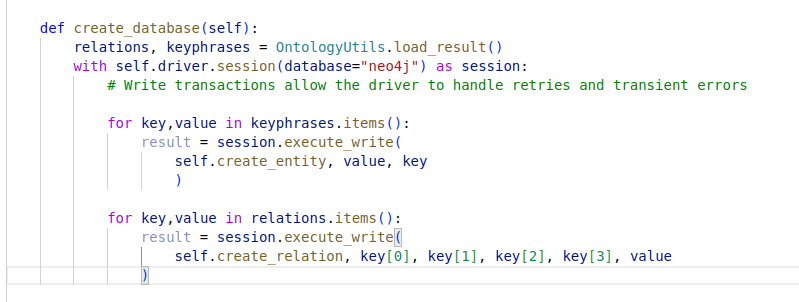
\includegraphics[scale=0.5]{../images/createdatabase}
    \end{center}
	
	La generación de los nodos como entidades la realizamos con las siguientes consulta:
	
	 \begin{center}
		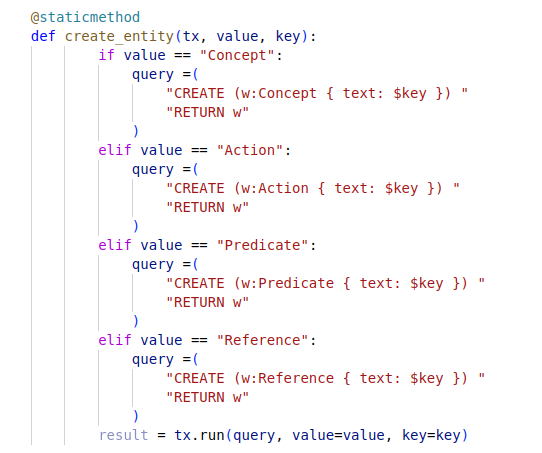
\includegraphics[scale=0.5]{../images/imageEntities}
	\end{center}
	
	Para la creación de las relaciones entre los nodos utilizamos la consulta:
	
	 \begin{center}
		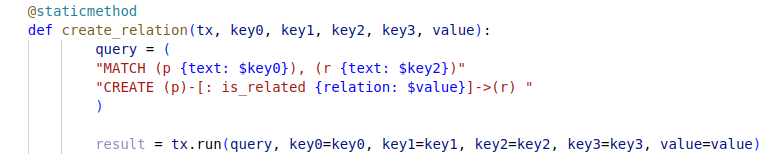
\includegraphics[scale=0.5]{../images/imageRelations}
	\end{center}

	El método a continuaci\'on realiza una consulta para conocer las causas de alguna enfermedad de interés:
	
	\begin{center}
		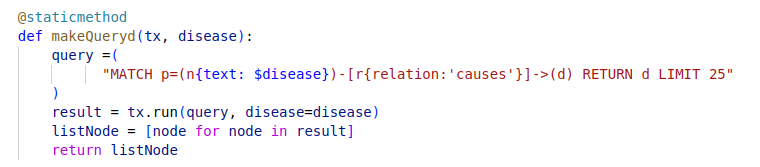
\includegraphics[scale=0.5]{../images/imageQuery}
	\end{center}

	En esta imagen podemos ver los resultado obtenidos al realizar la consulta para conocer las causas del covid-19:
	
	\begin{center}
		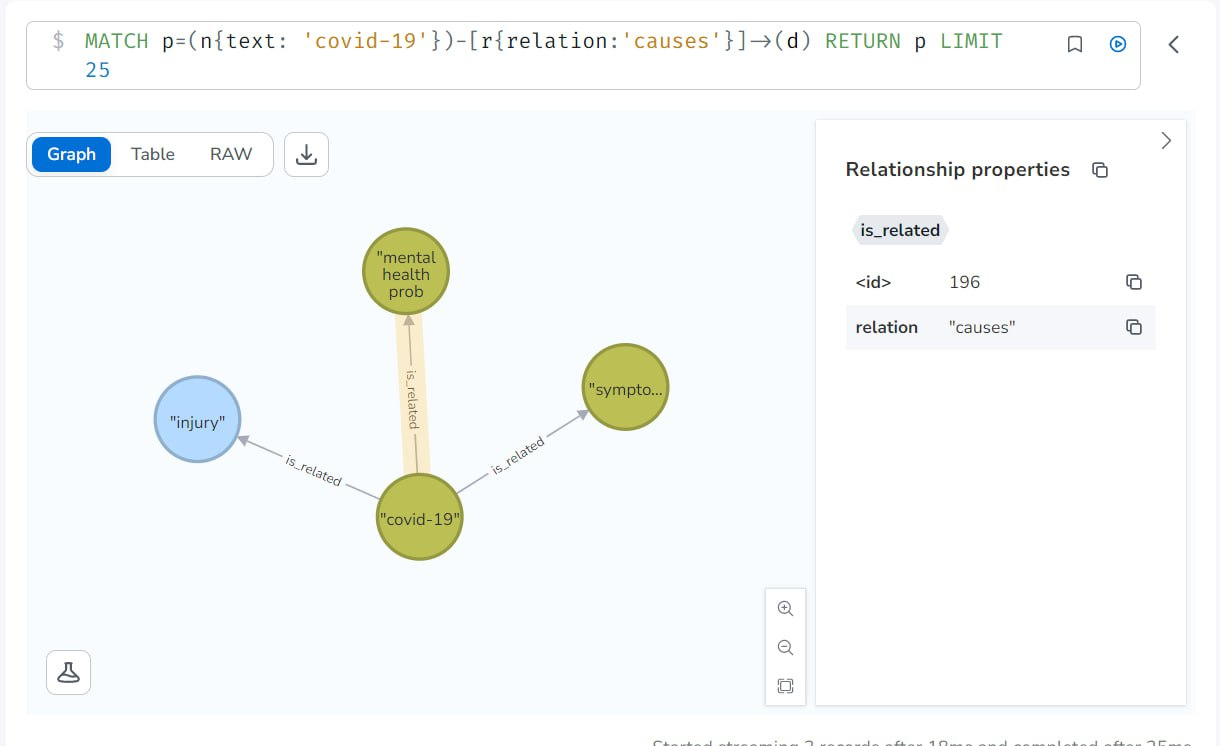
\includegraphics[scale=0.5]{../images/imagecons}
		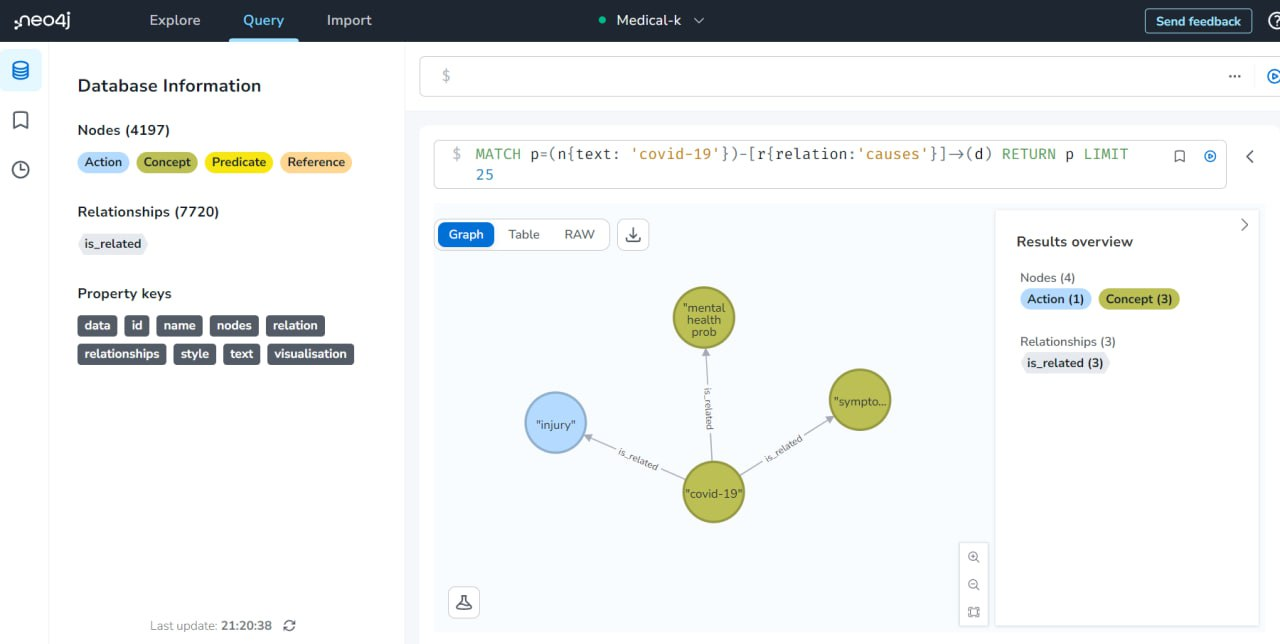
\includegraphics[scale=0.5]{../images/imagecons1}
		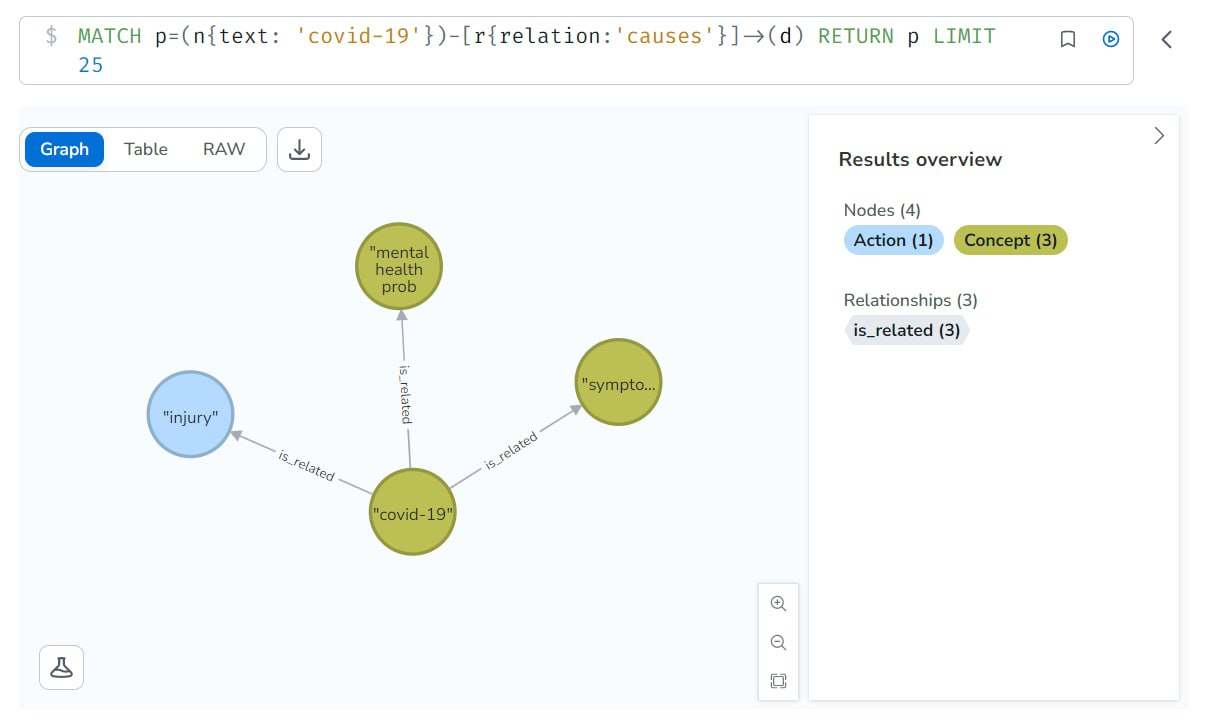
\includegraphics[scale=0.5]{../images/imageconsulta}
	\end{center}

	\section{Resultados}
	
	\selectlanguage{spanish}
	\begin{table}[htb]
		\centering
		\begin{tabular}{|c|c|c|c|c|}
			\hline
			\textbf{Modelo} & \textbf{Problema} & \textbf{Precisi\'on} & \textbf{Recobrado} & \textbf{F1} \\
			\hline
			\multirow{3}{*}{\textbf{BiLSTM}} & NER & 0.5583 & 0.5613 & 0.5598 \\
			\cline{2-5}
			& RE & 0.06451 & 0.03317 & 0.04381 \\
			\cline{2-5}
			& NER + RE & 0.36909 & 0.30406 & 0.3334 \\
			\hline
		\textbf{BERT} & NER & 1.0 & 0.8375 & 0.455782 \\
			\hline
			\multirow{2}{*}{\textbf{T5}} & NER & 0.535304 & 0.551253 & 0.397562 \\
			\cline{2-5}
			& RE & 0.68838 & 0.1129 & 0.09699 \\
			\hline
			\multirow{3}{*}{\textbf{GPT3}} & NER & 0.41744 & 0.32445 & 0.36512 \\
			\cline{2-5}
			& RE & 0.11374 & 0.061068 & 0.07947 \\
			\cline{2-5}
			& NER + RE & 0.2969 & 0.19602 & 0.23617 \\
			\hline
			\textbf{BiLSTM (NER) + T5 (RE)} & NER + RE & 0.6327 & 0.6327 & 0.6327 \\
			\hline
			
		\end{tabular}
		\caption{Comparaci\'on de los resultados de los modelos.}
		\label{resultados}
	\end{table}
	 \todo{hacer referencia a medidas}
	\todo{Verificar medidas T5 y LSTM + T5}
	
	
	\begin{figure}[htb]
		\centering
		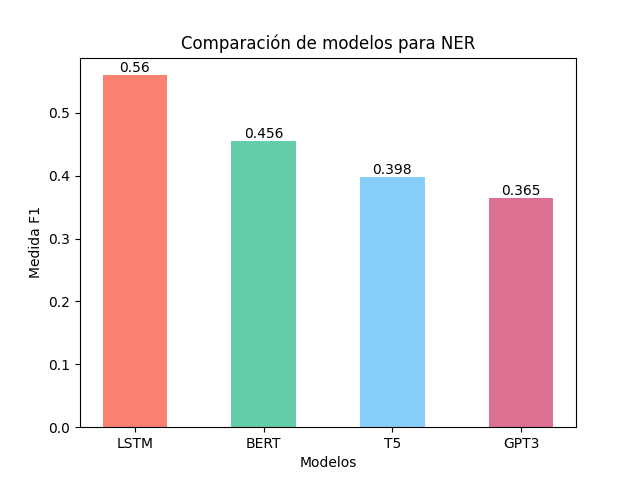
\includegraphics[scale=0.6]{../images/NER_bar}
		\caption{Gr\'afica de barra con los valores de la medida F1 de los modelos evaluados para el problema NER.}
		\label{NER}
	\end{figure}

		\begin{figure}[htb]
		\centering
		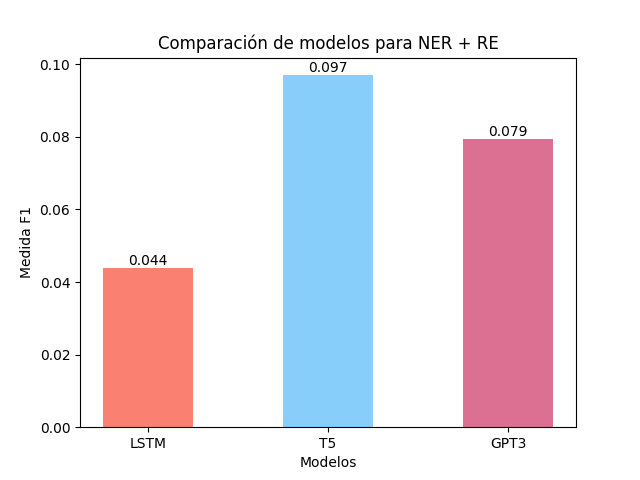
\includegraphics[scale=0.6]{../images/RE_bar}
		\caption{Gr\'afica de barra con los valores de la medida F1 de los modelos evaluados para el problema RE.}
		\label{RE}
	\end{figure}

	
	\begin{figure}[htb]
		\centering
		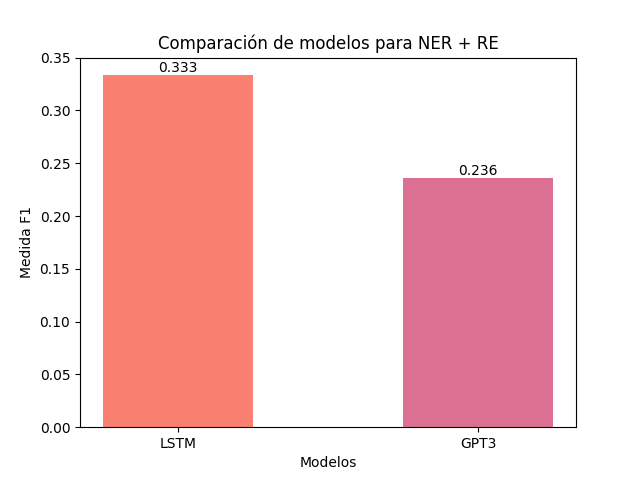
\includegraphics[scale=0.6]{../images/NER_RE_bar}
		\caption{Gr\'afica de barra con los valores de la medida F1 de los modelos evaluados para el problema NER + RE.}
		\label{NR}
	\end{figure}
	
	\section{Conclusiones}
	
	En conclusión, los resultados de nuestras experimentaciones demostraron la efectividad de los modelos de aprendizaje profundo, específicamente BiLSTM y T5, en la tarea de extracción de conocimiento a partir de textos médicos. En la tarea de extracción de entidades nombradas (NER), el modelo BiLSTM sobresalió con un puntaje F1 de 0.56, demostrando su habilidad para capturar y utilizar la información contextual en la identificación de entidades en el texto.
	
	Por otro lado, para la tarea de extracción de relaciones (RE), el modelo T5 se destacó con un puntaje F1 de 0.63. La superioridad de T5 en esta tarea se puede atribuir a su capacidad para entender y generar texto, lo que es esencial para identificar y clasificar las relaciones entre entidades en el texto.
	
	En términos de rendimiento general, la combinación de BiLSTM y T5 resultó ser la más eficaz, logrando un puntaje F1 de 0.63. Esto sugiere que, aunque los modelos individuales pueden ser eficaces para tareas específicas, la combinación de diferentes enfoques y técnicas puede llevar a un rendimiento mejorado.
	
	Estos resultados subrayan la capacidad del modelo T5 para llevar a cabo tareas de extracción de conocimiento. Aunque BiLSTM demostró ser eficaz en la tarea de NER, T5 demostró una versatilidad superior, siendo capaz de manejar tanto tareas de NER como de RE de manera efectiva. Esto demuestra el potencial de T5 y modelos similares para la extracción de conocimiento a partir de textos, y sugiere direcciones prometedoras para futuras investigaciones y desarrollos en este campo.
	
	\section{Recomendaciones}
	
	Las siguientes son algunas recomendaciones para futuras investigaciones y mejoras en este proyecto:
	
	\begin{itemize}
		\item Experimentar con modelos más nuevos y potentes: Aunque T5 ha demostrado ser eficaz en nuestras pruebas, existen modelos de lenguaje más nuevos y más potentes que podrían ser explorados para mejorar aún más la extracción de conocimiento. Modelos como GPT-3 de OpenAI, o modelos como BERT de Google y RoBERTa de Facebook, que utilizan la técnica de Transformer, pueden proporcionar un rendimiento mejorado.
		\item Mejora de los datos de entrenamiento: Aunque los modelos de aprendizaje profundo son potentes, su rendimiento depende en gran medida de la calidad de los datos de entrenamiento. Podría ser beneficioso invertir más tiempo y recursos en la mejora de los datos de entrenamiento, como la limpieza de los datos, la eliminación de sesgos y la adición de más ejemplos de entrenamiento.
		\item Pruebas con diferentes combinaciones de modelos: Los resultados indican que la combinación de BiLSTM y T5 fue la más eficaz para la tarea completa de extracción de conocimiento. Esto sugiere que la combinación de diferentes modelos y técnicas podría ser una estrategia eficaz. Futuras investigaciones podrían explorar diferentes combinaciones de modelos y técnicas para mejorar aún más el rendimiento.
		\item Explorar técnicas de preprocesamiento de texto avanzadas: Antes de alimentar el texto a los modelos de aprendizaje profundo, podría ser útil explorar técnicas avanzadas de preprocesamiento de texto, como la lematización, la eliminación de stopwords y la codificación de entidades.
		\item Incorporación de conocimientos del dominio: En tareas específicas del dominio, como la extracción de conocimientos médicos, la incorporación de conocimientos del dominio puede mejorar el rendimiento del modelo. Futuras investigaciones podrían explorar formas de incorporar conocimientos médicos en los modelos para mejorar la extracción de entidades y relaciones.
	\end{itemize}
	
   	
	\begin{thebibliography}
		a
		\bibitem{introduction} Cormen, Thomas H. y otros. \emph{Introduction to Algorithms}. 
		The MIT Press.
		4ta Edici\'on.		
		Cambridge, Massachusetts.
		2022.
	\end{thebibliography}
\end{document}


